\section{Grouped Cross-Validation Results and Protocol Verification}
The three-fold hyperparameter search is now supplemented by an explicit \emph{five-fold} grouped cross-validation audit. The latter is not an alternative name for the original grid: it is an additional experiment in which the already selected SVM settings and the fixed Naive Bayes baseline are fit afresh five times. The training portion alone (19,213 records) is partitioned with \texttt{StratifiedGroupKFold(n\_splits=5, shuffle=True, random\_state=20261026)}. Every fold refits the TF-IDF vectorizer from scratch. The validation partition (2,399 rows) and reserved final test partition (2,388 rows) are excluded from these five-fold splits.

\begin{table}[H]\centering\caption{Observed composition of the five validation folds}\label{tab:fold-audit}\small\begin{tabular}{rrrrrr}\toprule
Fold & CV records & Valid & Suspicious & Spam & Group overlap\\\midrule
1 & 3,842 & 1,281 & 1,281 & 1,280 & 0\\
2 & 3,842 & 1,281 & 1,281 & 1,280 & 0\\
3 & 3,842 & 1,281 & 1,281 & 1,280 & 0\\
4 & 3,844 & 1,281 & 1,283 & 1,280 & 0\\
5 & 3,843 & 1,280 & 1,283 & 1,280 & 0\\\bottomrule
\end{tabular}\end{table}
The held-out partition in each fold has approximately one-fifth of the training rows, with between 1,510 and 1,511 scenario-family IDs. Each fold's corresponding training side has between 6,041 and 6,042 families, and the measured overlap is \textbf{zero} in all five cases. This documents identifier-level separation, but does not prove that word choices or writing templates are independent across groups.

\begin{table}[H]\centering\caption{Measured five-fold Macro-F1 by algorithm}\label{tab:fivefold}\small\begin{tabular}{rrrr}\toprule
Fold & Linear SVM Macro-F1 & Naive Bayes Macro-F1 & Training rows\\\midrule
1 & 1.00000 & 0.99323 & 15,371\\
2 & 1.00000 & 0.99323 & 15,371\\
3 & 1.00000 & 0.99297 & 15,371\\
4 & 1.00000 & 0.99115 & 15,369\\
5 & 1.00000 & 0.99167 & 15,370\\\midrule
Mean & \textbf{1.00000} & \textbf{0.99245} & --\\
Sample SD & 0.00000 & 0.00097 & --\\\bottomrule
\end{tabular}\end{table}

\begin{figure}[H]\centering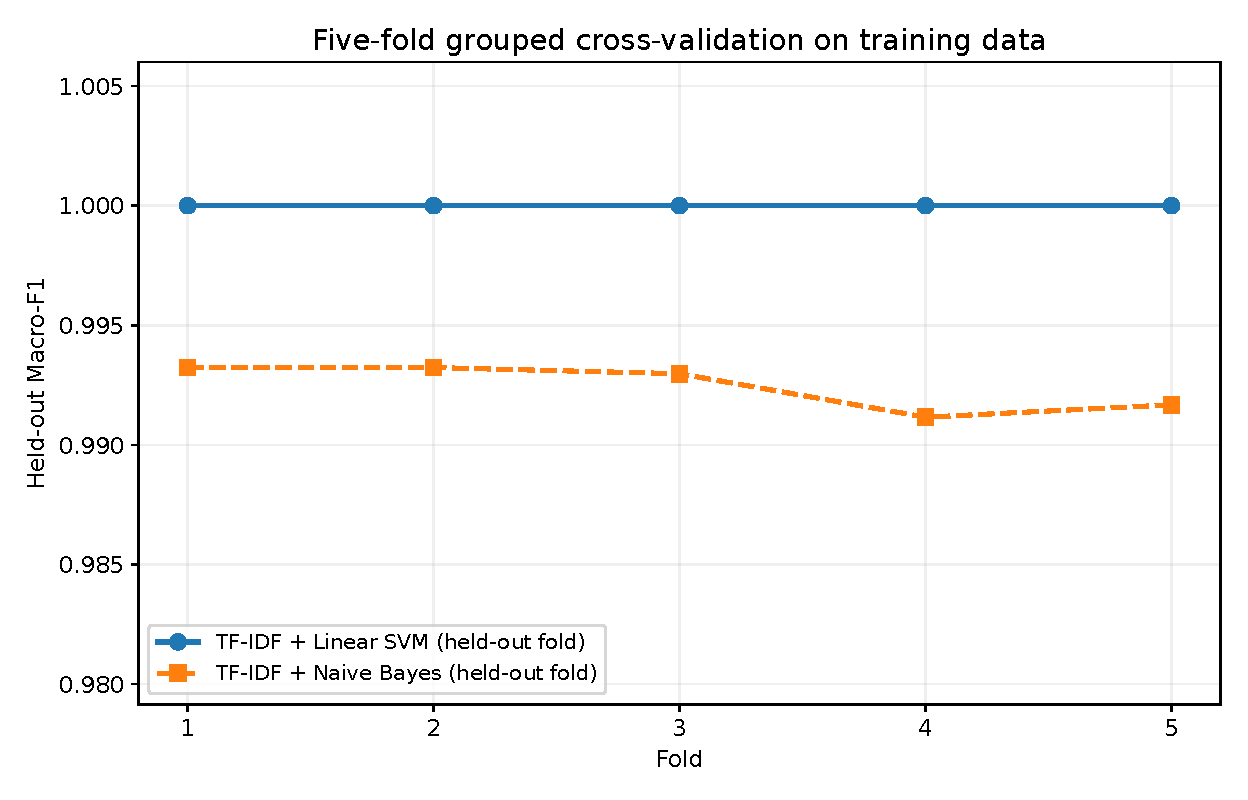
\includegraphics[width=.90\textwidth]{figures/m3_grouped_fivefold_scores.pdf}\caption{Fold-level Macro-F1 for the selected SVM and the Naive Bayes baseline. The horizontal SVM series is evidence of a ceiling on these generator-derived folds, not a universal error rate of zero.}\end{figure}
The agreement between the three-fold grid and the additional five-fold result indicates that the model's exceptionally high generated-data score is not an accident of one particular partition. It does \emph{not} imply that the generator has produced five genuinely different linguistic distributions. Because all folds are derived from one generation process, stable scores could also indicate class-specific lexical conventions that generalize across the generator's own scenario families.

\section{Hyperparameter Optimization: All Eighteen Configurations}
In the original grid, the Cartesian product $C\in\{0.1,1,10\}$, word $n$-grams $\{(1,1),(1,2)\}$ and \texttt{min\_df}$\in\{2,5,10\}$ produced 18 settings; \texttt{max\_df=0.95} and sublinear TF weighting were held fixed. The three-fold model-selection metric was mean held-out Macro-F1. Every configuration obtained 1.0000 on this particular generation-derived grid, with standard deviation 0.0000. Consequently, the default deterministic tie resolution produced $C=0.1$, unigrams and \texttt{min\_df=2}. This is a selection rule, not evidence that $C=0.1$ is inherently better for future complaints.
\begin{figure}[H]\centering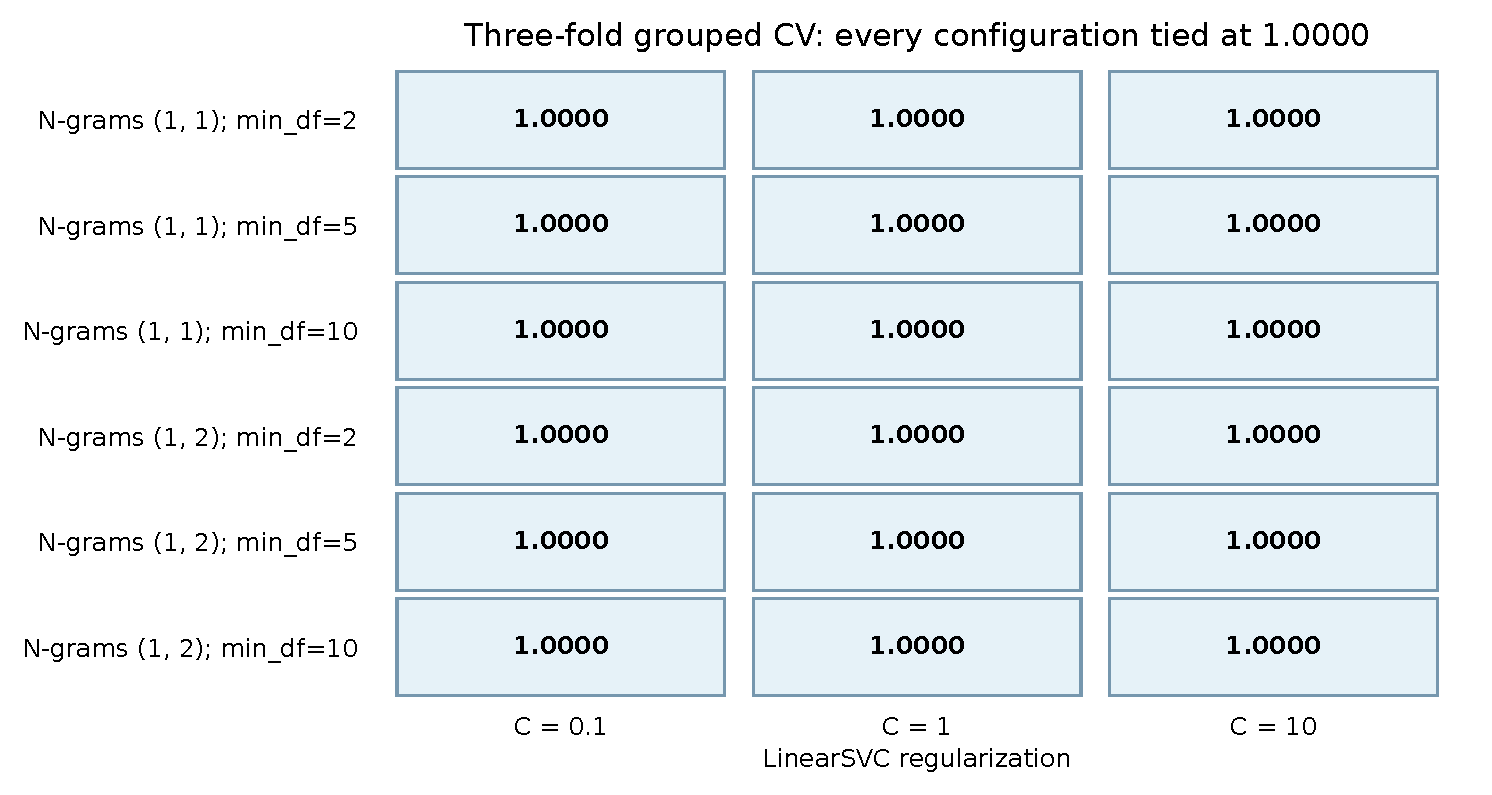
\includegraphics[width=.98\textwidth]{figures/m3_hyperparameter_matrix.pdf}\caption{The complete three-fold grouped SVM grid (18 combinations) as a labeled score matrix. Uniform values explicitly demonstrate a \emph{hyperparameter discrimination ceiling}.}\label{fig:grid-heatmap}\end{figure}

To help reproduce the evaluation, the exact 18 rows are archived in \path{results/hyperparameter_grid_v2.csv}. A sensitivity claim would require configurations to produce different performance values on an informative development distribution. The absence of such variation cannot be interpreted as proof that tuning is unnecessary.

\section{Validation Set: Error Counts and Confusion Matrices}
After training on all 19,213 training messages, the selected SVM and fixed Naive Bayes baseline were evaluated on 2,399 validation messages. The final generated test partition was not used in the additional the present study experiments.
\begin{table}[H]\centering\caption{Held-out validation metrics with explicit mistake counts}\label{tab:valid-summary}\small\begin{tabular}{lrrrrr}\toprule
Model & Accuracy & Macro-precision & Macro-recall & Macro-F1 & Errors\\\midrule
Linear SVM & 1.0000 & 1.0000 & 1.0000 & 1.0000 & 0\\
Naive Bayes & 0.9921 & 0.9923 & 0.9921 & 0.9921 & 19\\\bottomrule
\end{tabular}\end{table}
\begin{figure}[H]\centering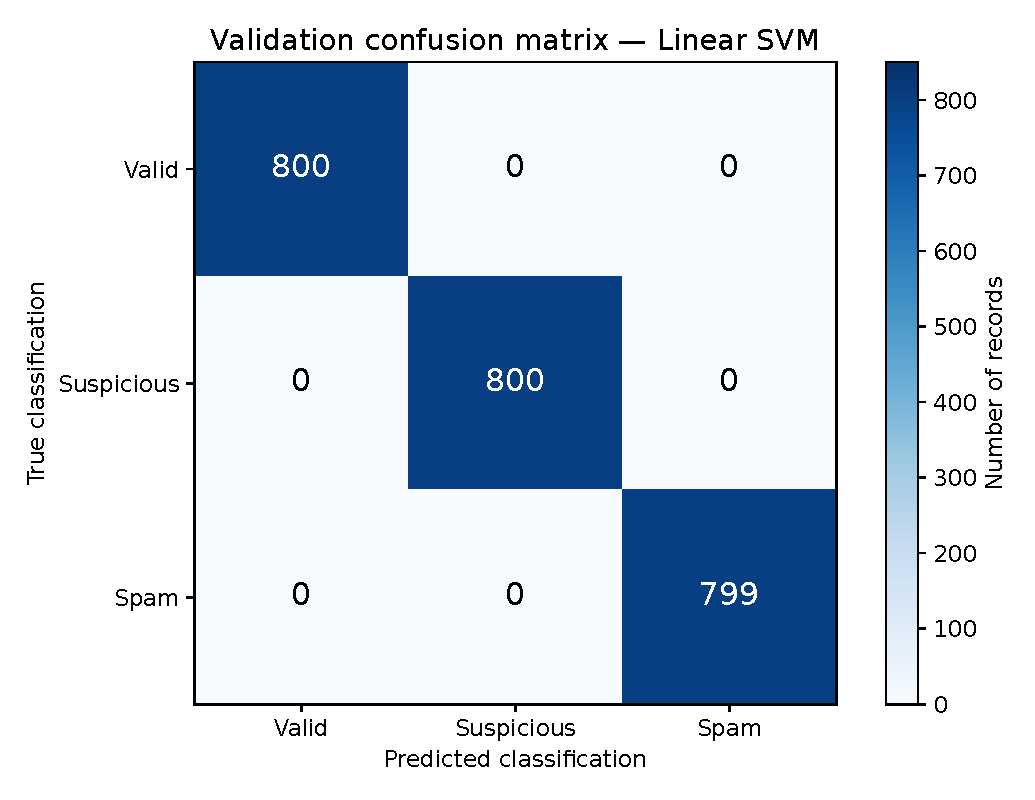
\includegraphics[width=.86\textwidth]{figures/m3_validation_confusion_svm.pdf}\caption{Linear SVM validation confusion matrix. Axes show true and predicted categories; diagonal counts are 800 Valid, 800 Suspicious, and 799 Spam.}\end{figure}
\begin{figure}[H]\centering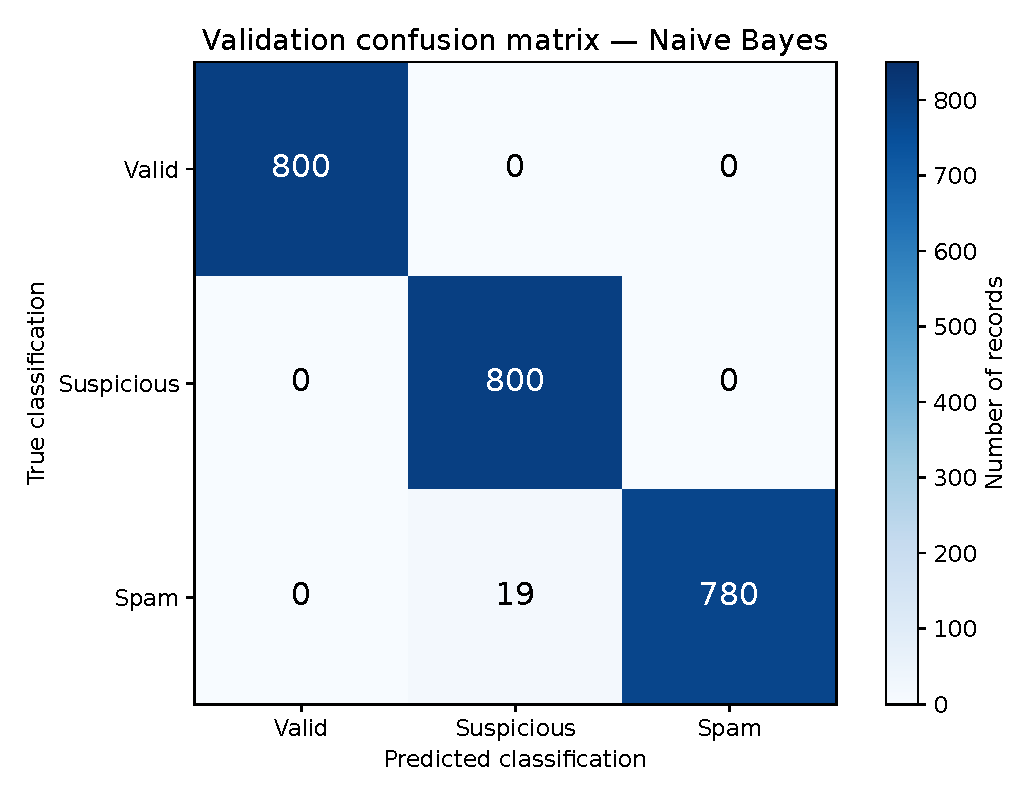
\includegraphics[width=.86\textwidth]{figures/m3_validation_confusion_nb.pdf}\caption{Naive Bayes validation confusion matrix. All 19 errors are Spam narratives predicted as Suspicious under the recorded label ordering Valid, Suspicious, Spam.}\end{figure}

\begin{table}[H]\centering\caption{Naive Bayes validation performance by classification}\small\begin{tabular}{lrrrr}\toprule Class & Precision & Recall & F1 & Support\\\midrule
Valid & 1.0000 & 1.0000 & 1.0000 & 800\\
Suspicious & 0.9768 & 1.0000 & 0.9883 & 800\\
Spam & 1.0000 & 0.9762 & 0.9880 & 799\\\bottomrule
\end{tabular}\end{table}
These errors are relevant operationally: some non-complaint messages might be sent to the clarification queue rather than removed as Spam. However, the dataset's ``Suspicious'' label describes clarification needs and must not be equated with dishonesty. Because the labels were generated from predefined rules and have not yet undergone an independent human reliability study, a perfect SVM validation score cannot be treated as an estimate of field performance.


\section{Recorded Final Synthetic Test and Paired Model Comparison}
\label{sec:m2-recorded-test}
The original experiment stored an additional evaluation on the 2,388-record test split. This test partition was not used by the later five-fold grouped validation supplement, but it \emph{was already evaluated} in the original run. The values in Table~\ref{tab:m2test} are copied from \path{results/model_results_v2.json}; they are not newly measured predictions.
\begin{table}[H]\centering\caption{Recorded 2,388-row synthetic test metrics (same records, both models)}\label{tab:m2test}\small\begin{tabular}{lrrrrrr}\toprule
Model & Accuracy & Macro-Prec. & Macro-Recall & Macro-F1 & Weighted-F1 & Errors\\\midrule
Linear SVM & 1.0000 & 1.0000 & 1.0000 & 1.0000 & 1.0000 & 0\\
Naive Bayes & 0.9916 & 0.9918 & 0.9917 & 0.9916 & 0.9916 & 20\\\bottomrule
\end{tabular}\end{table}
\begin{table}[H]\centering\caption{Per-class precision, recall and F1 on the recorded synthetic test partition}\small
\begin{tabular}{llrrr}\toprule Model & True class & Precision & Recall & F1\\\midrule
SVM & Valid & 1.0000 & 1.0000 & 1.0000\\
SVM & Suspicious & 1.0000 & 1.0000 & 1.0000\\
SVM & Spam & 1.0000 & 1.0000 & 1.0000\\
Naive Bayes & Valid & 1.0000 & 1.0000 & 1.0000\\
Naive Bayes & Suspicious & 0.9753 & 1.0000 & 0.9875\\
Naive Bayes & Spam & 1.0000 & 0.9750 & 0.9874\\\bottomrule
\end{tabular}\end{table}
The recorded SVM test confusion matrix is diagonal with supports (796, 791, 801) for Valid, Suspicious and Spam, respectively; therefore all three of its precision, recall and F1 values are 1.0000 on the same synthetic test. The Naive Bayes test confusion matrix is $\bigl(\begin{smallmatrix}796&0&0\\0&791&0\\0&20&781\end{smallmatrix}\bigr)$ (row=true class, column=predicted class). The Naive Bayes per-class test F1 scores are 1.0000 (Valid), 0.9875 (Suspicious) and 0.9874 (Spam). Twenty actual Spam entries were called Suspicious; no Valid text was called Spam in the recorded test.

\begin{table}[H]\centering\caption{Exact McNemar analysis reconstructed from test correctness totals}\label{tab:m2mcnemar}\small\begin{tabular}{lrr}\toprule
Baseline result / SVM result & SVM correct & SVM wrong\\\midrule
Naive Bayes correct & 2,368 & 0\\
Naive Bayes wrong & 20 & 0\\\bottomrule
\end{tabular}\end{table}
The paired test table is determinable here from the common 2,388-case split, the SVM's zero errors and the baseline's 20 errors, even though row-level test predictions were not saved in the present package. With discordant $b=0,c=20$, the exact two-sided McNemar $p=0.00000191 <0.05$ supports a difference in classifier error incidence \emph{on this synthetic benchmark}. It does not demonstrate superiority for naturally authored, independently annotated complaints. The original test has been inspected, so all future feature or threshold decisions require a fresh external test; no additional ``unseen test'' status is claimed for these 2,388 cases.

\section{Assigned-Language Subgroup Analysis}
The validation split is evaluated by the metadata assigned during generation. Language-group tags are used only for \emph{analysis}, not passed to the classifier. The validation set contains 594 Bisaya, 616 Filipino, 596 English and 593 Mixed messages. Table~\ref{tab:languages} reveals the observed subgroup distribution of model scores.
\begin{table}[H]\centering\caption{Validation Macro-F1 by assigned language group}\label{tab:languages}\small\begin{tabular}{lrrr}\toprule
Language & N & Linear SVM & Naive Bayes\\\midrule
Bisaya & 594 & 1.0000 & 0.9933\\
Filipino & 616 & 1.0000 & 0.9934\\
English & 596 & 1.0000 & 0.9899\\
Mixed & 593 & 1.0000 & 0.9917\\\bottomrule
\end{tabular}\end{table}
These within-generator subgroup scores do not establish linguistic fairness or success with naturally occurring code-switching. The generation metadata explicitly identifies that language verification has not been completed. Independent Cebuano and Filipino language review would therefore remain necessary before claiming reliable multilingual operation.

\section{Training-Size Learning Curve and Optimization-Time Loss}
A learning curve was measured for the selected SVM using training sizes 1,921; 3,842; 6,724; 9,606; 14,409; and 19,213. The training Macro-F1 was nearly 1.0 throughout; held-out validation Macro-F1 started at 0.998749 for 1,921 training rows and reached 1.0000 at 3,842 rows. See Figure~\ref{fig:learning-original} in the earlier section. As training and validation performance saturate extremely early, this experiment does not justify a claim that the classifier will adapt well to new linguistic behaviors merely by increasing the number of similarly generated records.

\texttt{LinearSVC} does not provide a documented epoch-level training-history stream. Accordingly, the original research ran a separate \texttt{SGDClassifier(loss=hinge)} experiment to record fifteen training passes and training/validation multiclass hinge loss. This is a \emph{different estimator}, and its loss trajectory must never be presented as the optimization trace for the final LinearSVC. The recorded training loss fell from 0.272574 at epoch 1 to 0.009421 at epoch 15, while validation loss decreased from 0.300816 to 0.012279. At the same time, validation Macro-F1 increased from 0.9624 to 0.9921, with some small non-monotonic fluctuations.
A decreasing loss without a persistent train/validation divergence indicates no strong \emph{epoch-wise} overfitting signal in this auxiliary run. It cannot address distribution shift between one synthetic generator and natural complaints. In particular, the unusually early learning-curve ceiling raises the possibility of artificial regularities that are easy for sparse linear models to recognize.

\section{Feature-Ablation and Shortcut Diagnostics}
To examine whether content-free cues explain part of the performance, a logistic regression baseline was trained on only two scalar inputs: token count and character count. It achieved 0.5494 accuracy and 0.5372 Macro-F1 on the fixed validation split. Although these numbers are far below the text classifiers, they are substantially above chance performance for a balanced three-class problem. This indicates that class-dependent message length and character count are predictive in the generated material and justify further attention to class-conditional sampling designs.

A separate exploratory model using character TF-IDF 3--5-grams and LinearSVC also achieved 1.0000 validation Macro-F1. This does \emph{not} provide evidence that character features improve transfer performance: the comparison uses the same generator-derived validation split and therefore inherits its limitations. It is included as a feature-boundary check only and must not be used retrospectively to choose the final model based on the reserved test data.
\begin{figure}[H]\centering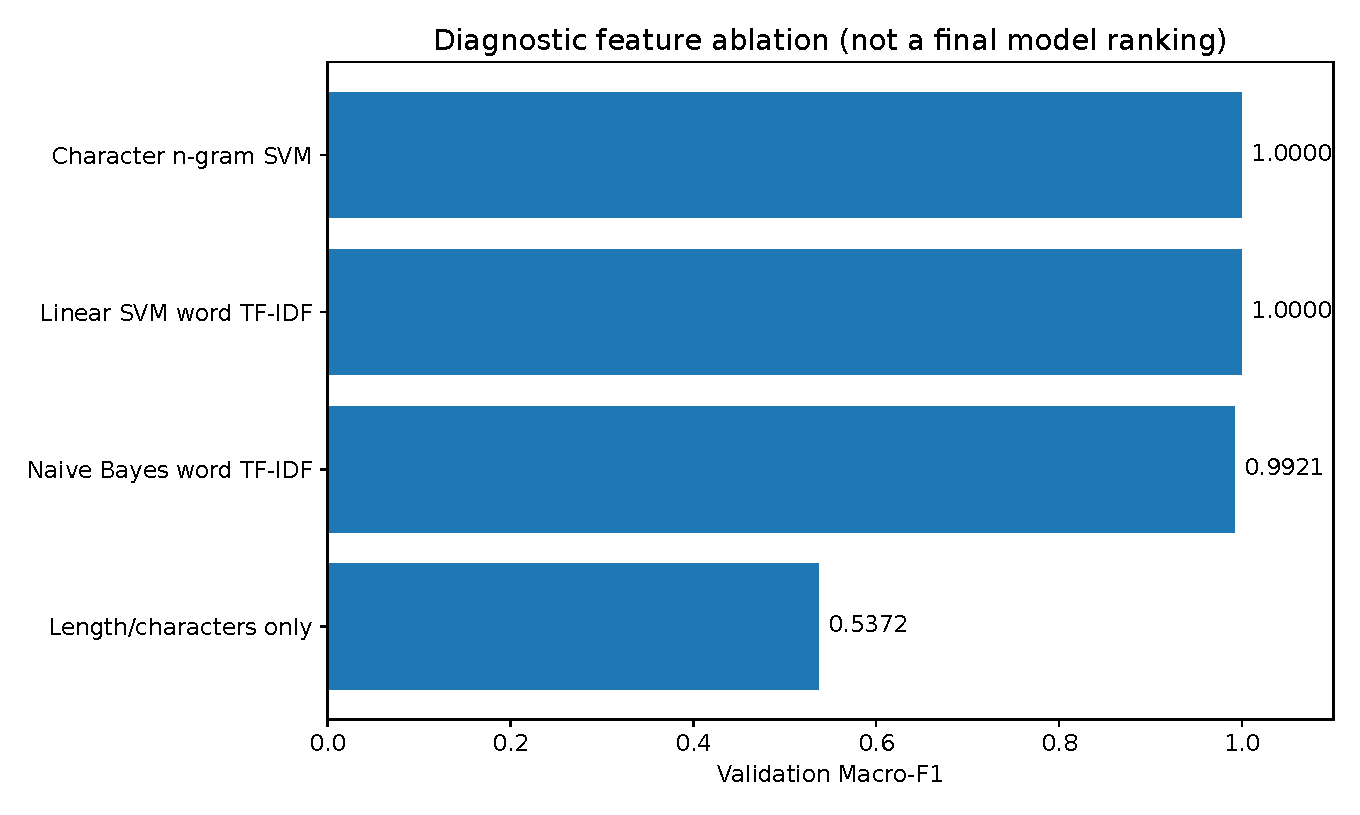
\includegraphics[width=.98\textwidth]{figures/m3_feature_ablation.pdf}\caption{Validation diagnostic comparison: message length alone, word-based models and exploratory character n-grams. Different feature availability tests what superficial cues can achieve, not semantic understanding.}\end{figure}

\section{Summary of Findings, Validity Threats, and Required Validation}
\textbf{Observed evidence.} The project can reproduce the planned 24,000-row corpus; uses 118 researcher-defined generation categories; fits TF-IDF within grouped folds; tests an 18-configuration SVM search; reports a five-fold group-based comparison against Naive Bayes; supplies fixed-validation confusion matrices and language comparisons; and presents both a sample-size learning curve and a genuine epoch-by-epoch auxiliary hinge-loss trace.

\textbf{Internal validity.} Recorded group overlap is zero within each five-fold split. Nevertheless, the groups are generated under common class-conditional narrative rules. Thus the folds are \emph{scenario-ID distinct} but not guaranteed to be lexically, syntactically or behaviorally independent. The original 18-way grid returning an identical score for every setting reinforces the need for more discriminating data and tests.

\textbf{Construct validity.} The system predicts researcher-defined three-way labels. These are not factual verdicts, legal findings or official barangay case outcomes. Synthetic narratives marked as human-unreviewed cannot establish inter-rater reliability. Simple abbreviations, missing nonessential fields, or an angry tone must not be conflated with suspicious intent.

\textbf{External validity.} the present study reports no deployment-stage administrator study, prospective human-in-the-loop adaptation trial, or blind population-based estimate. An appropriate next phase would pre-register a new independently constructed language-behavior test, obtain blinded expert review of difficult labels, audit urgent-case failure modes, and only then evaluate retrained candidates against an unchanged external benchmark. These activities remain future evaluation tasks rather than completed the present study results.
